\documentclass[tikz, crop, border = {2pt 2pt 2pt 2pt}]{standalone}

\usepackage{concmath-otf}
\usetikzlibrary{calc, angles, quotes, patterns}
\usetikzlibrary{decorations.pathreplacing, decorations.pathmorphing, calligraphy}

\begin{document}
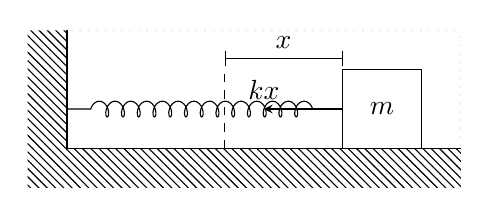
\begin{tikzpicture}
	\fill[even odd rule, pattern = north west lines] (-0.5, -0.5) rectangle (5, 1.5) (0, 0) rectangle (5, 1.5);
	\draw (0, 1.5) -- (0, 0) -- (5, 0);

	\node[draw, rectangle, minimum size = 1cm] (m) at (4, 0.5){$m$};
	\draw[decorate, decoration = {coil, amplitude = 0.1cm, segment length = 0.2cm, aspect = 0.6, pre length = 0.3cm, post length = 0.3cm}] (0, 0.5) -- (m);

	\draw[-stealth] (m) -- ++ (-1.5, 0) node[above]{$kx$};

	\draw[dashed] (2, 0) -- ++ (0, 1);

	\draw[shift = {(0, 4pt)}, |-|] (2, 1) -- node[above]{$x$} (3.5, 1);
\end{tikzpicture}
\end{document}
